% !TEX root = ../paper.tex
\section{Illustrations}						% 2-4 pages

\begin{figure}[H]
  \caption{Quadrotor dynamics \cite{Kumar:QuadrotorOverview} }
  \centering
    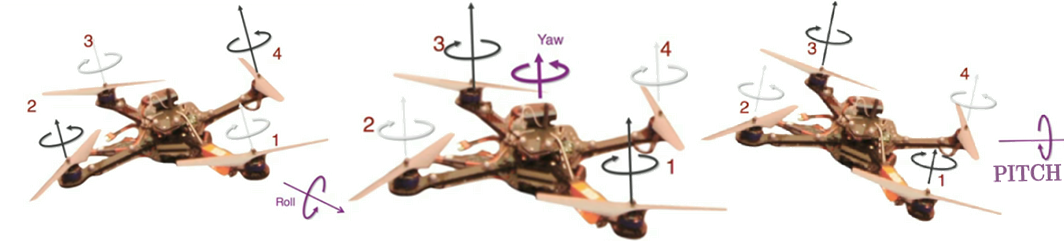
\includegraphics[width=\textwidth]{illustrations/quadcopter_diagram}
\end{figure}

\begin{figure}[h]
	\begin{minipage}{.5\textwidth}
		\caption{Mapping system breakdown}
		\centering
			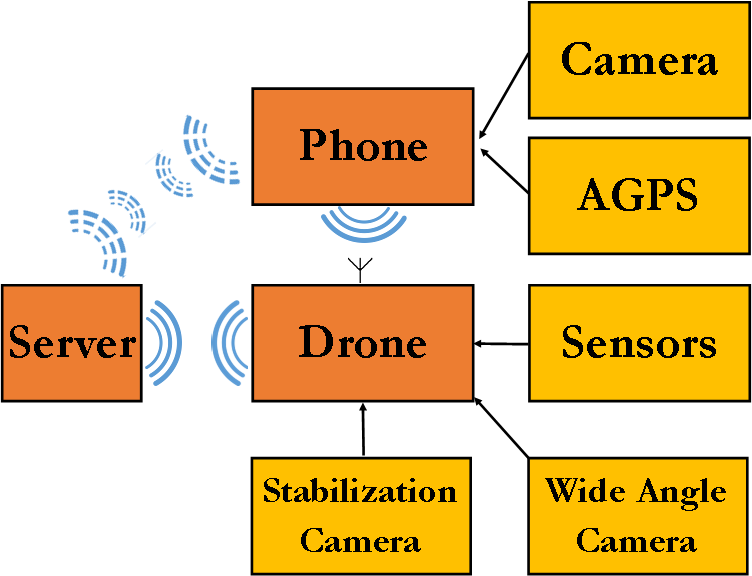
\includegraphics[width=0.95\linewidth]{illustrations/system_chart}
	\end{minipage}
	\begin{minipage}{.5\textwidth}
		\caption{Arduino interfacing with drone}
		\label{fig:ArduinoDrone}
		\centering
			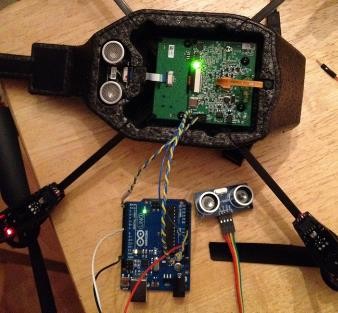
\includegraphics[width=0.95\linewidth]{illustrations/arduino_drone}
	\end{minipage}
\end{figure}

\begin{figure}[h]
	\begin{minipage}{.5\textwidth}
		\caption{Stitch from night-time UAV flyover}
		\label{fig:KennedySidewalk}
		\centering
			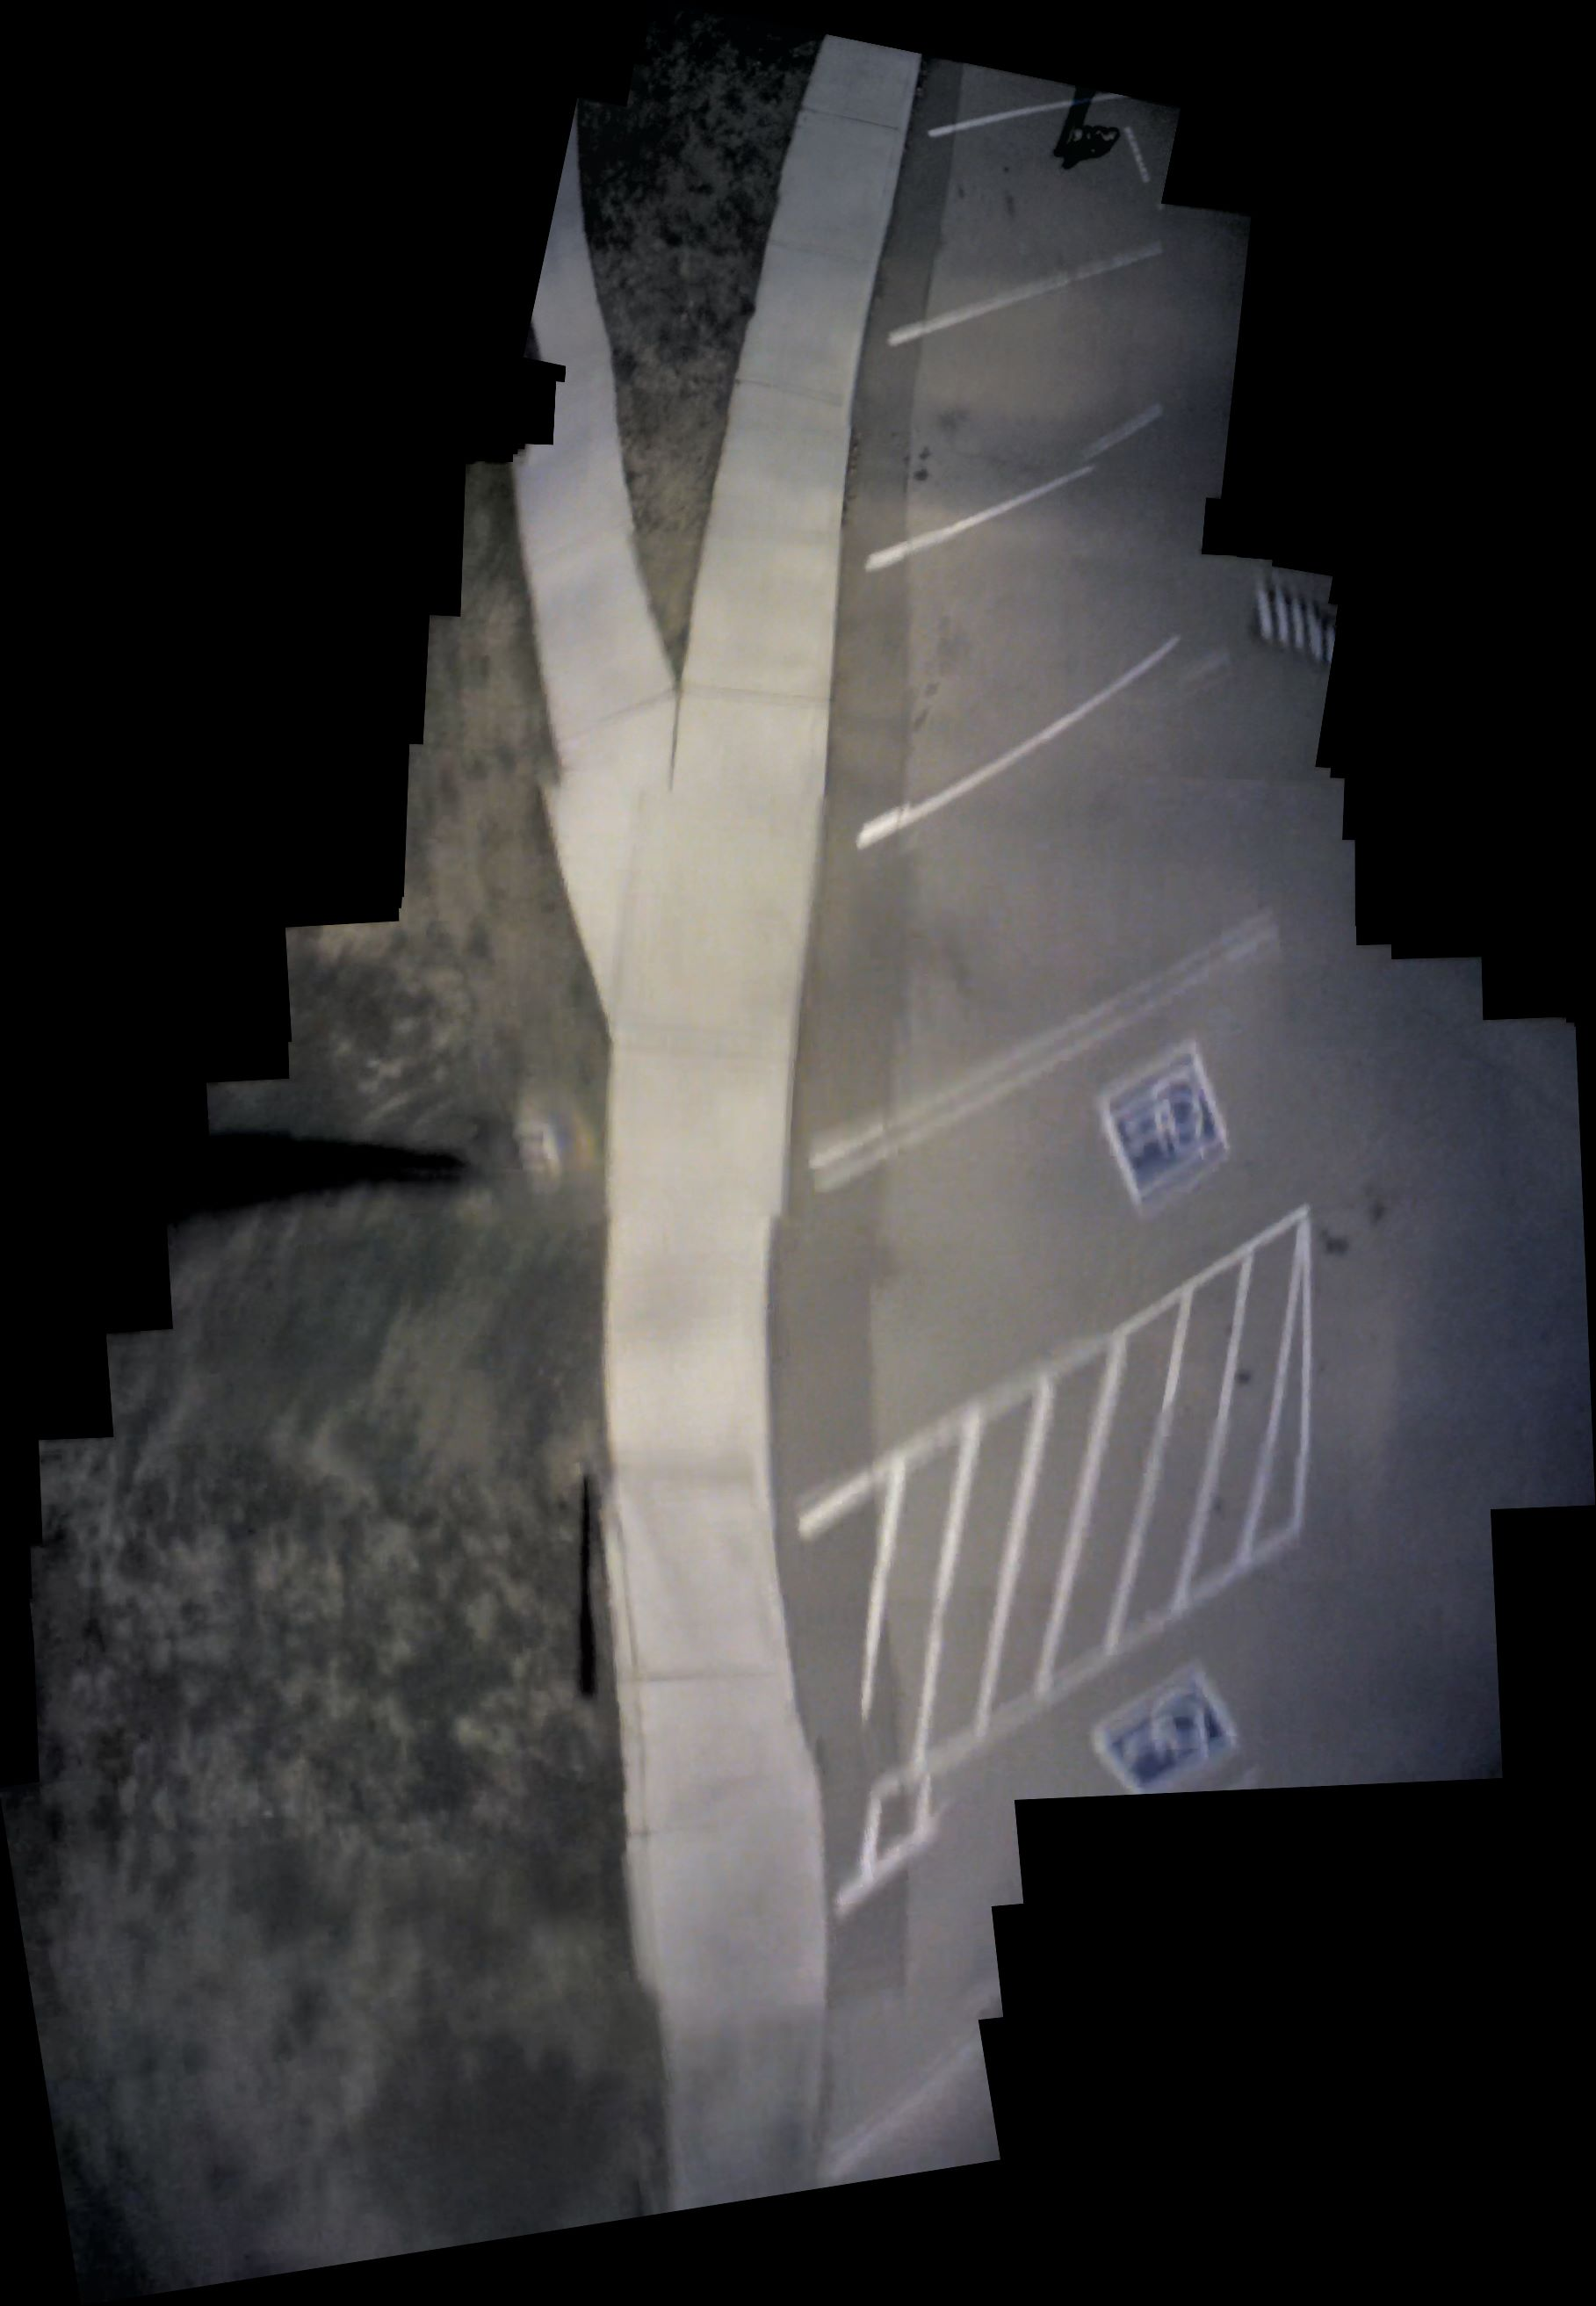
\includegraphics[width=0.95\linewidth]{illustrations/maps/KennedySidewalkStitch}
	\end{minipage}
	\begin{minipage}{.5\textwidth}
		\caption{Comparison of satellite and stitch quality}
		\label{fig:DebrisEarth}
		\centering
			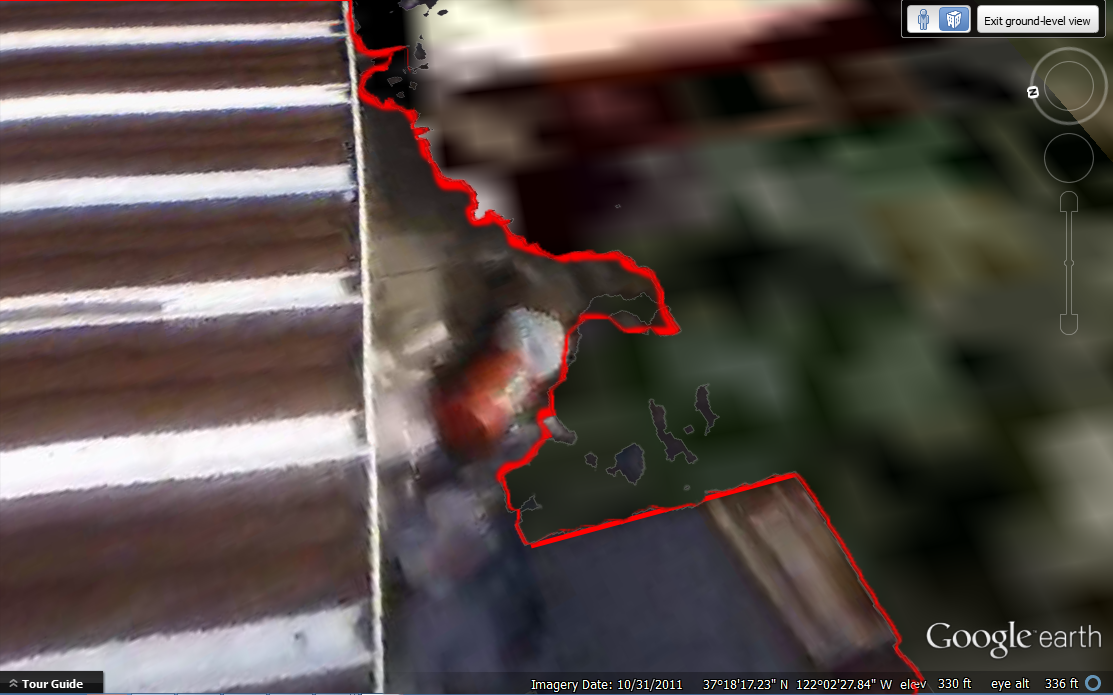
\includegraphics[width=0.95\linewidth]{illustrations/maps/debris}
		\linebreak
		\caption{Stitched image of a playground}
		\label{fig:Playground}
		\centering
			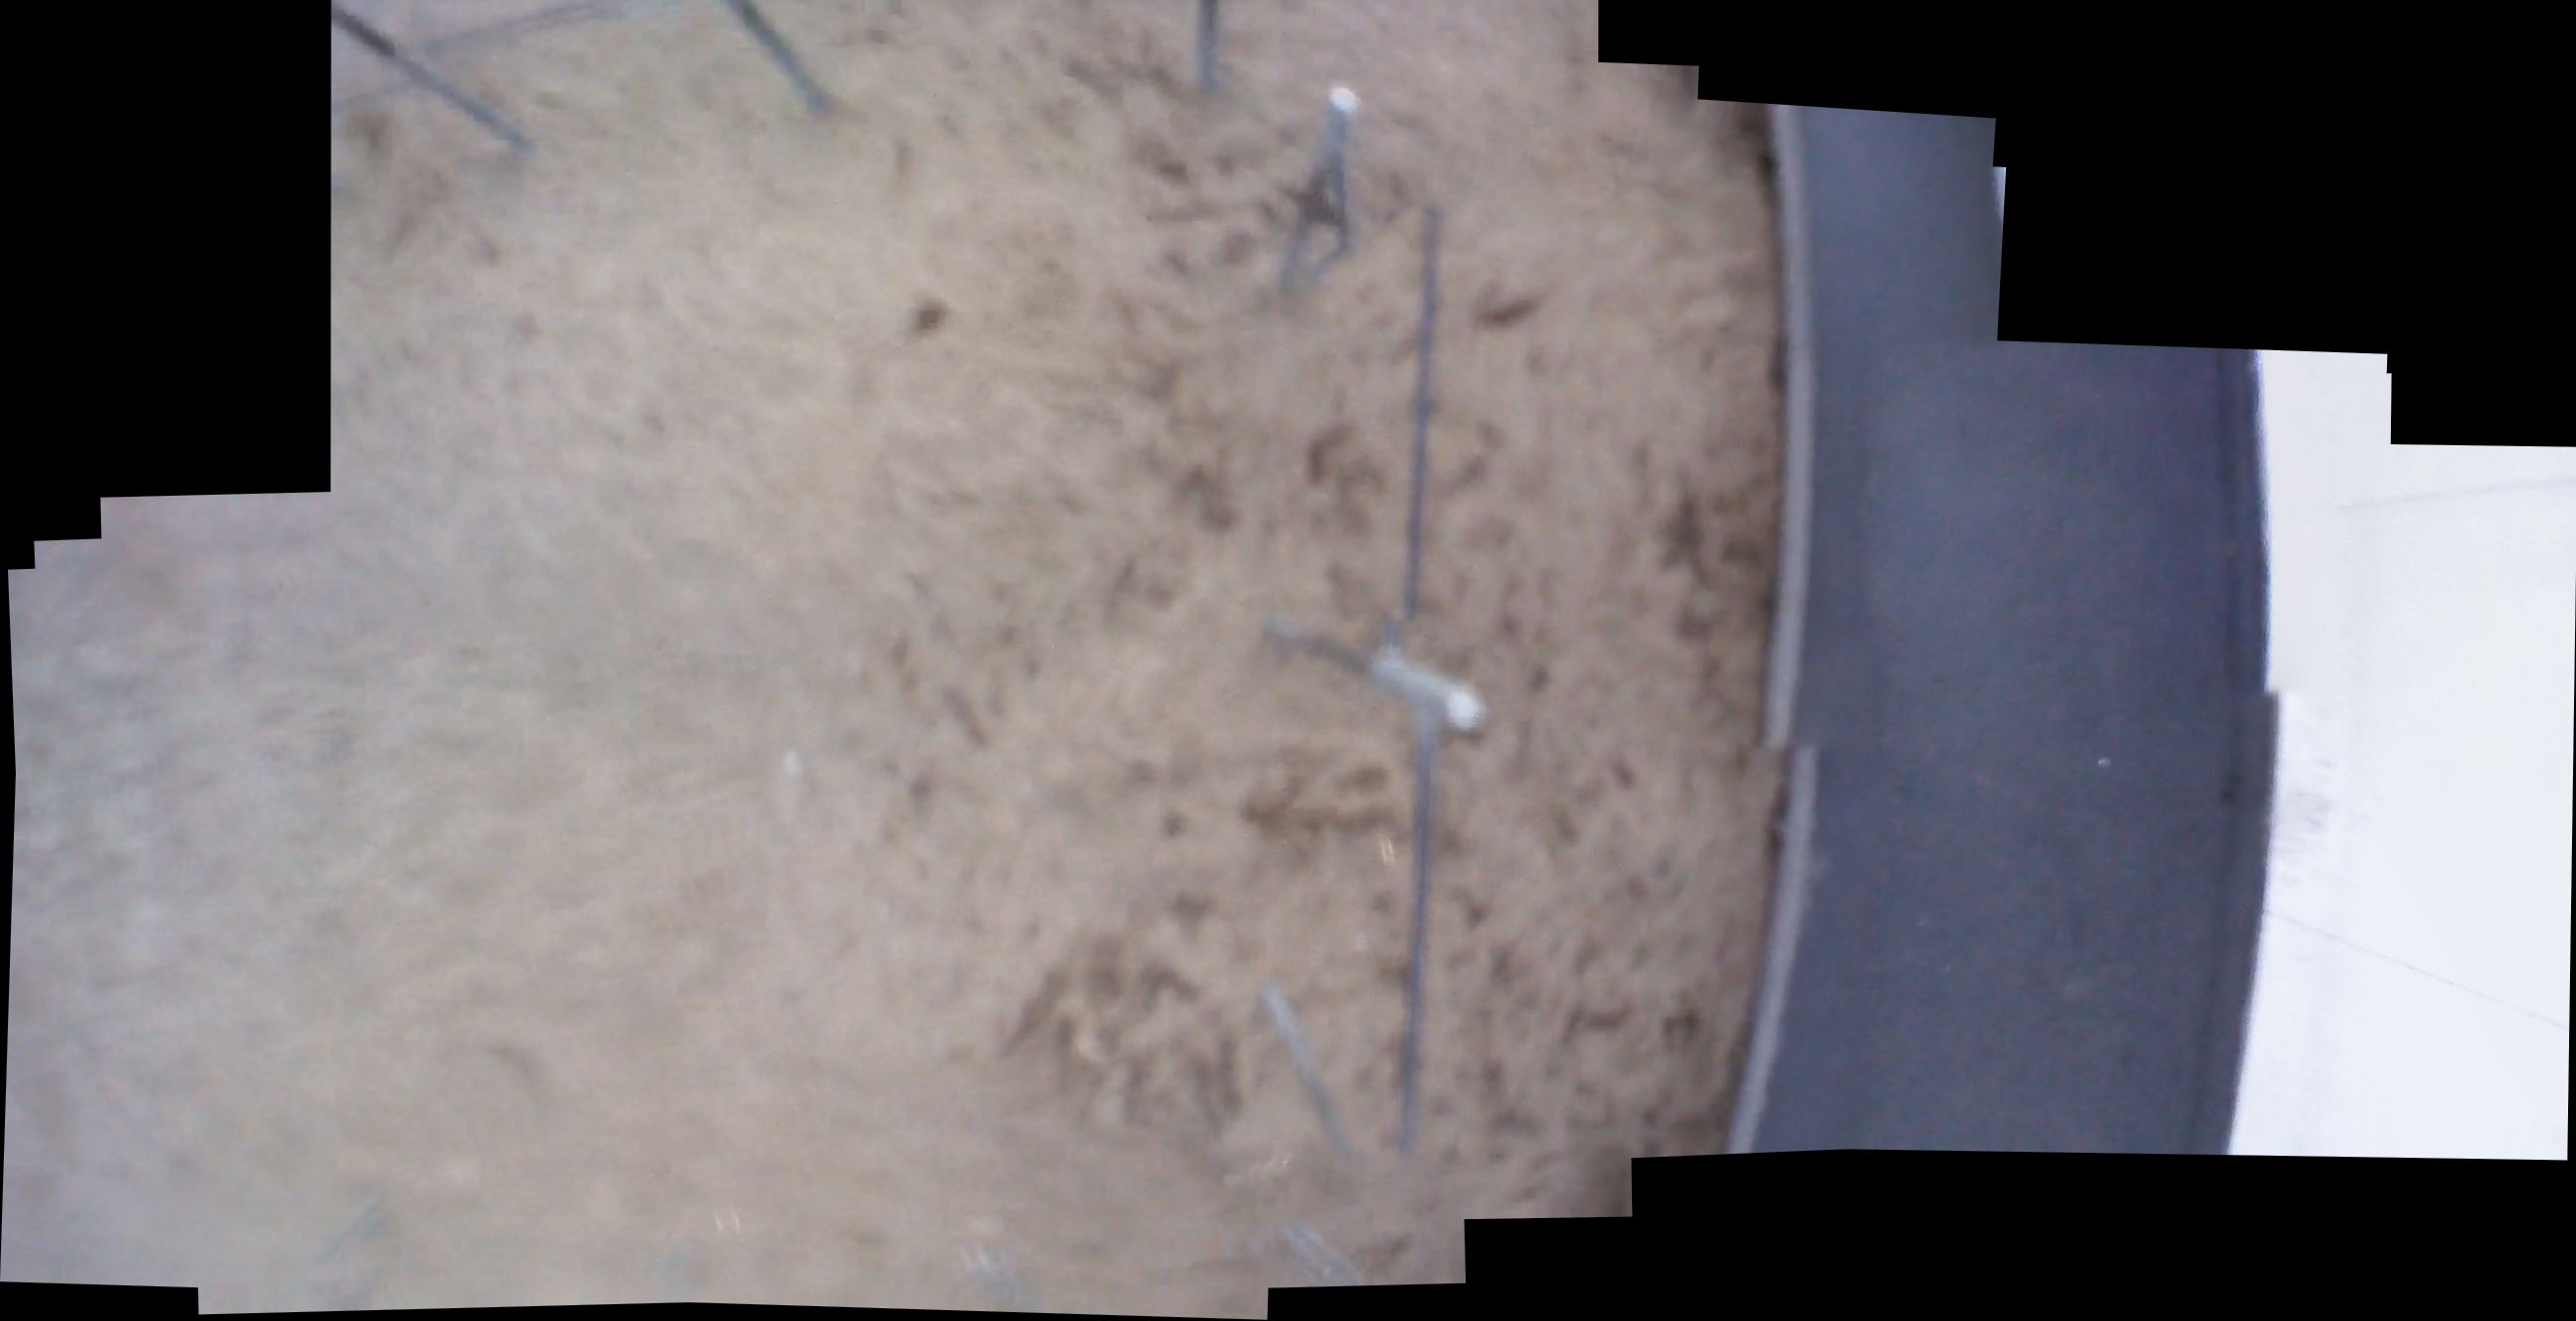
\includegraphics[width=0.95\linewidth]{illustrations/maps/tanbark_structures}
	\end{minipage}
\end{figure}
\clearpage
\begin{figure}[H]
	\caption{Map created from house flyover}
	\label{fig:HouseStitch}
	\centering
		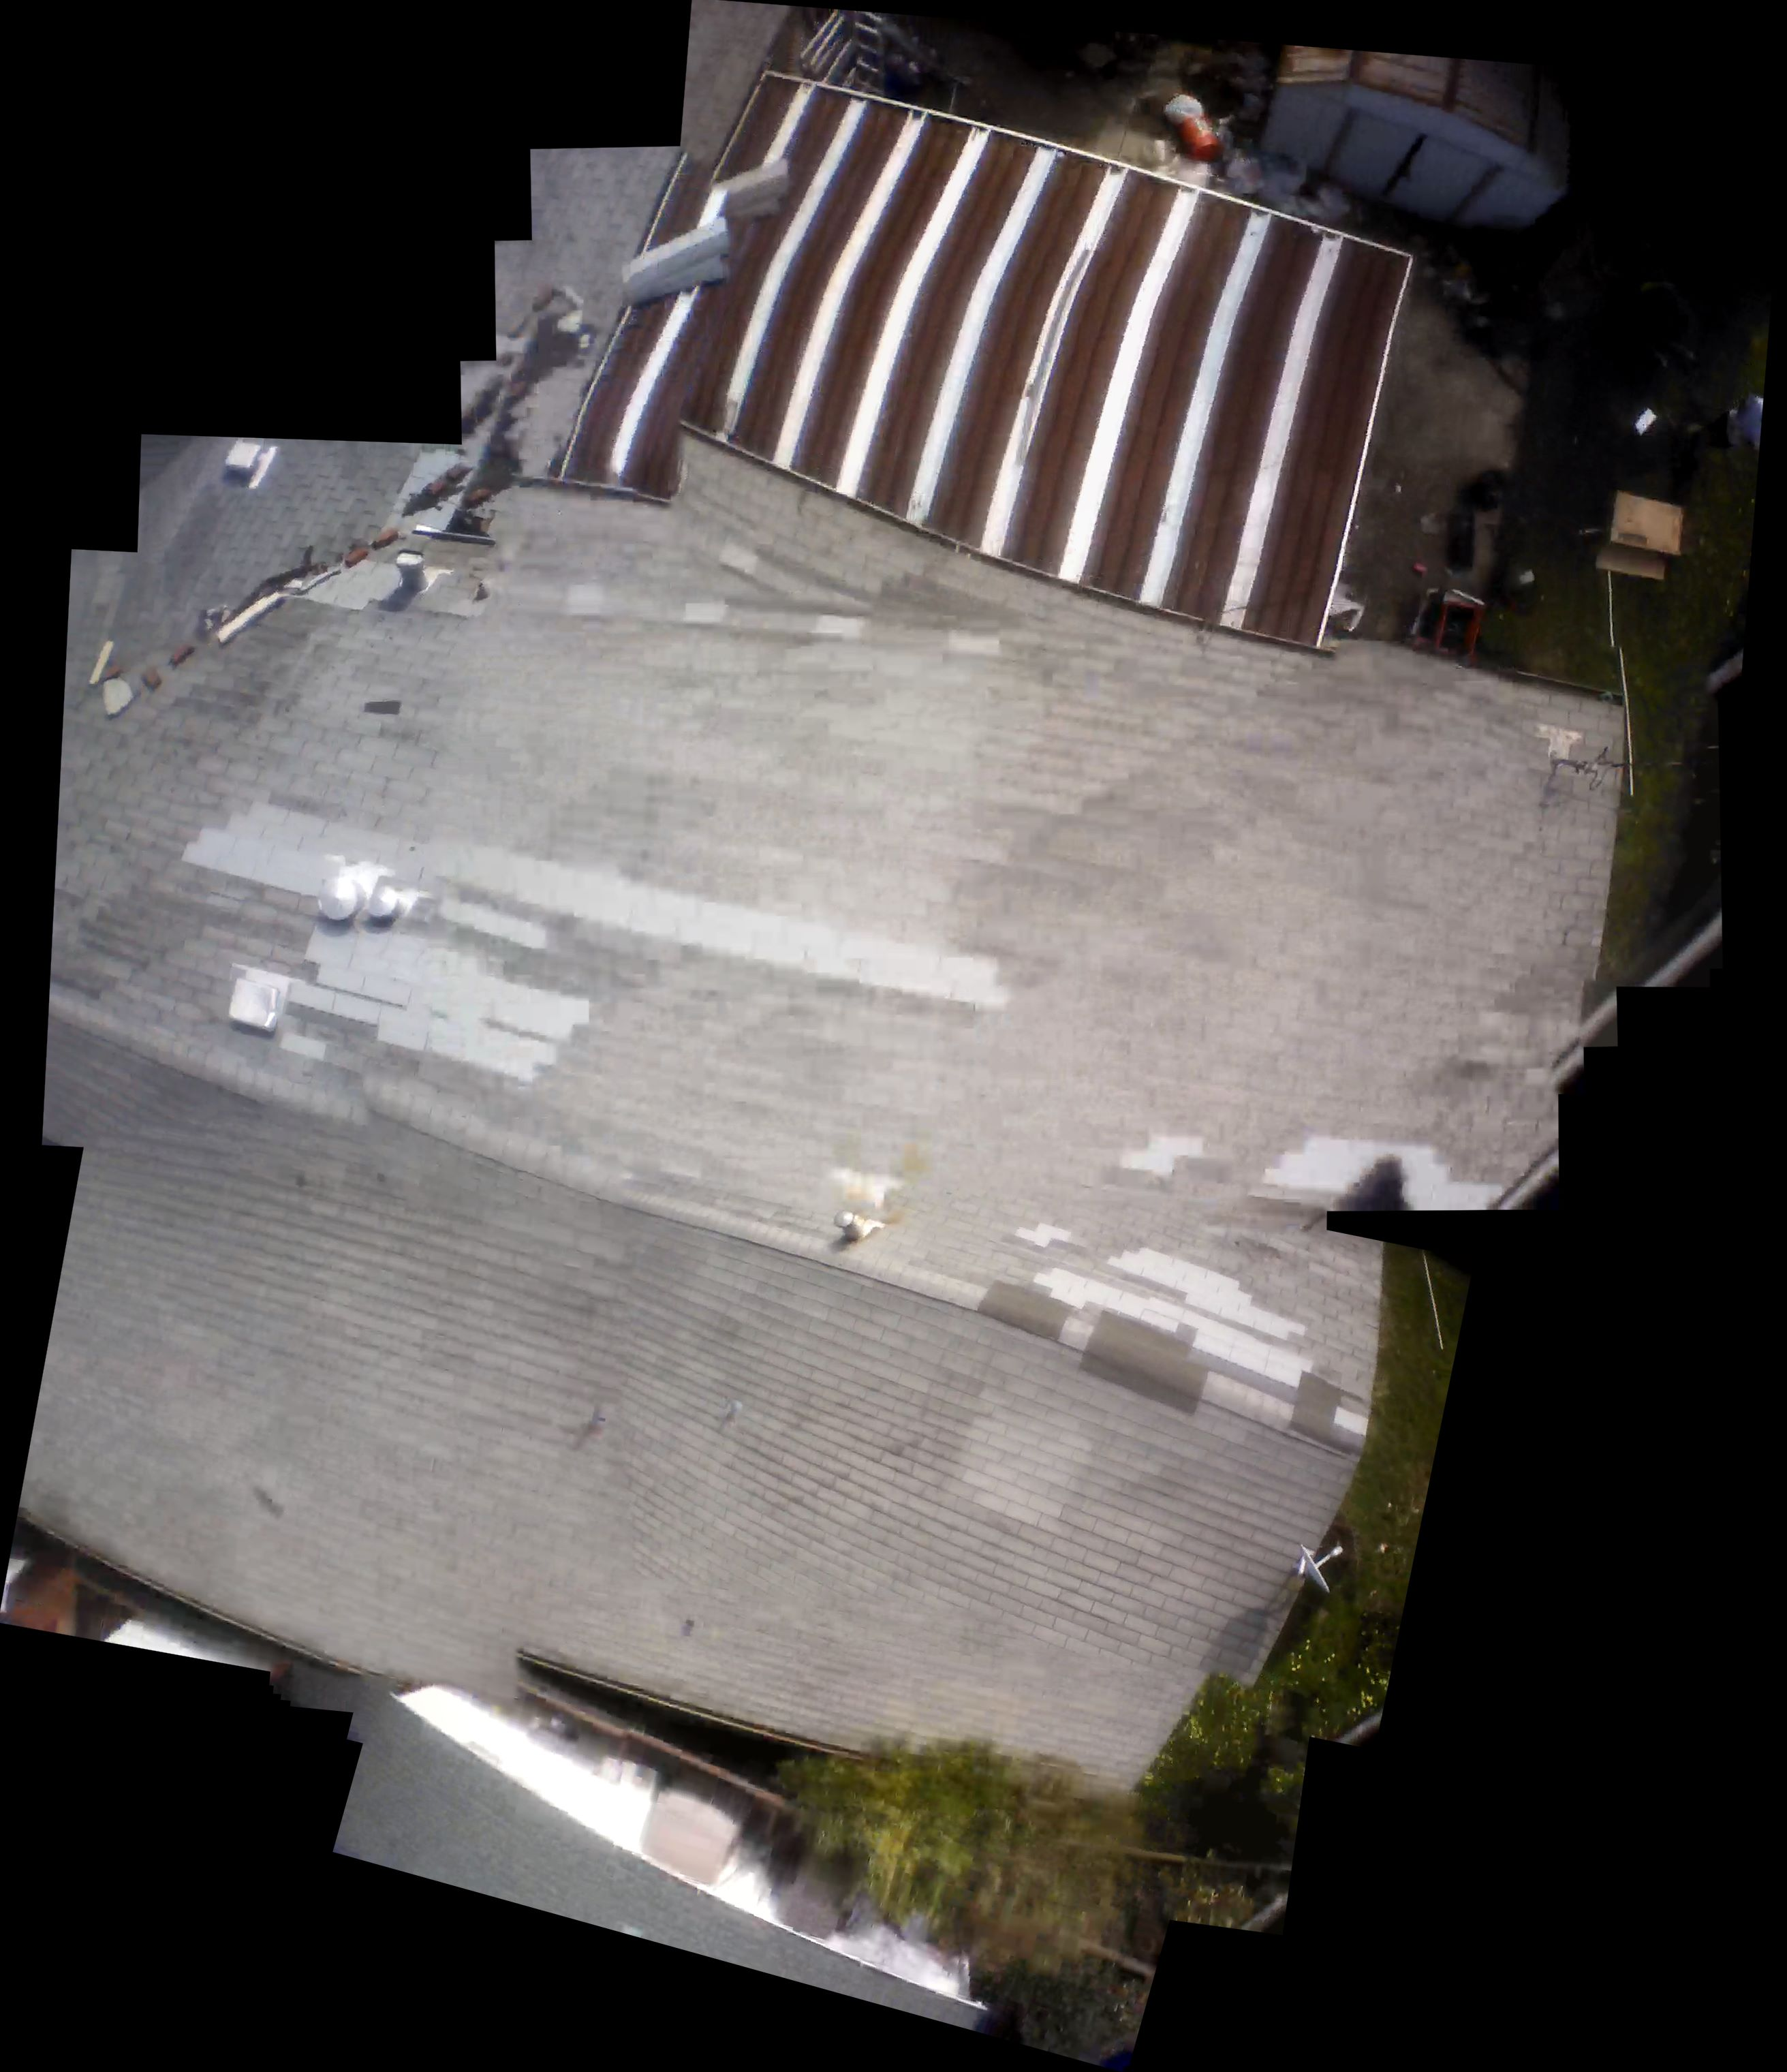
\includegraphics[width=\textwidth]{illustrations/maps/house}
\end{figure}

\begin{figure}[H]
  \caption{Panoramic stitched image from 720 p front camera above rooftops}
  \label{fig:StellingStitch}
  \centering
    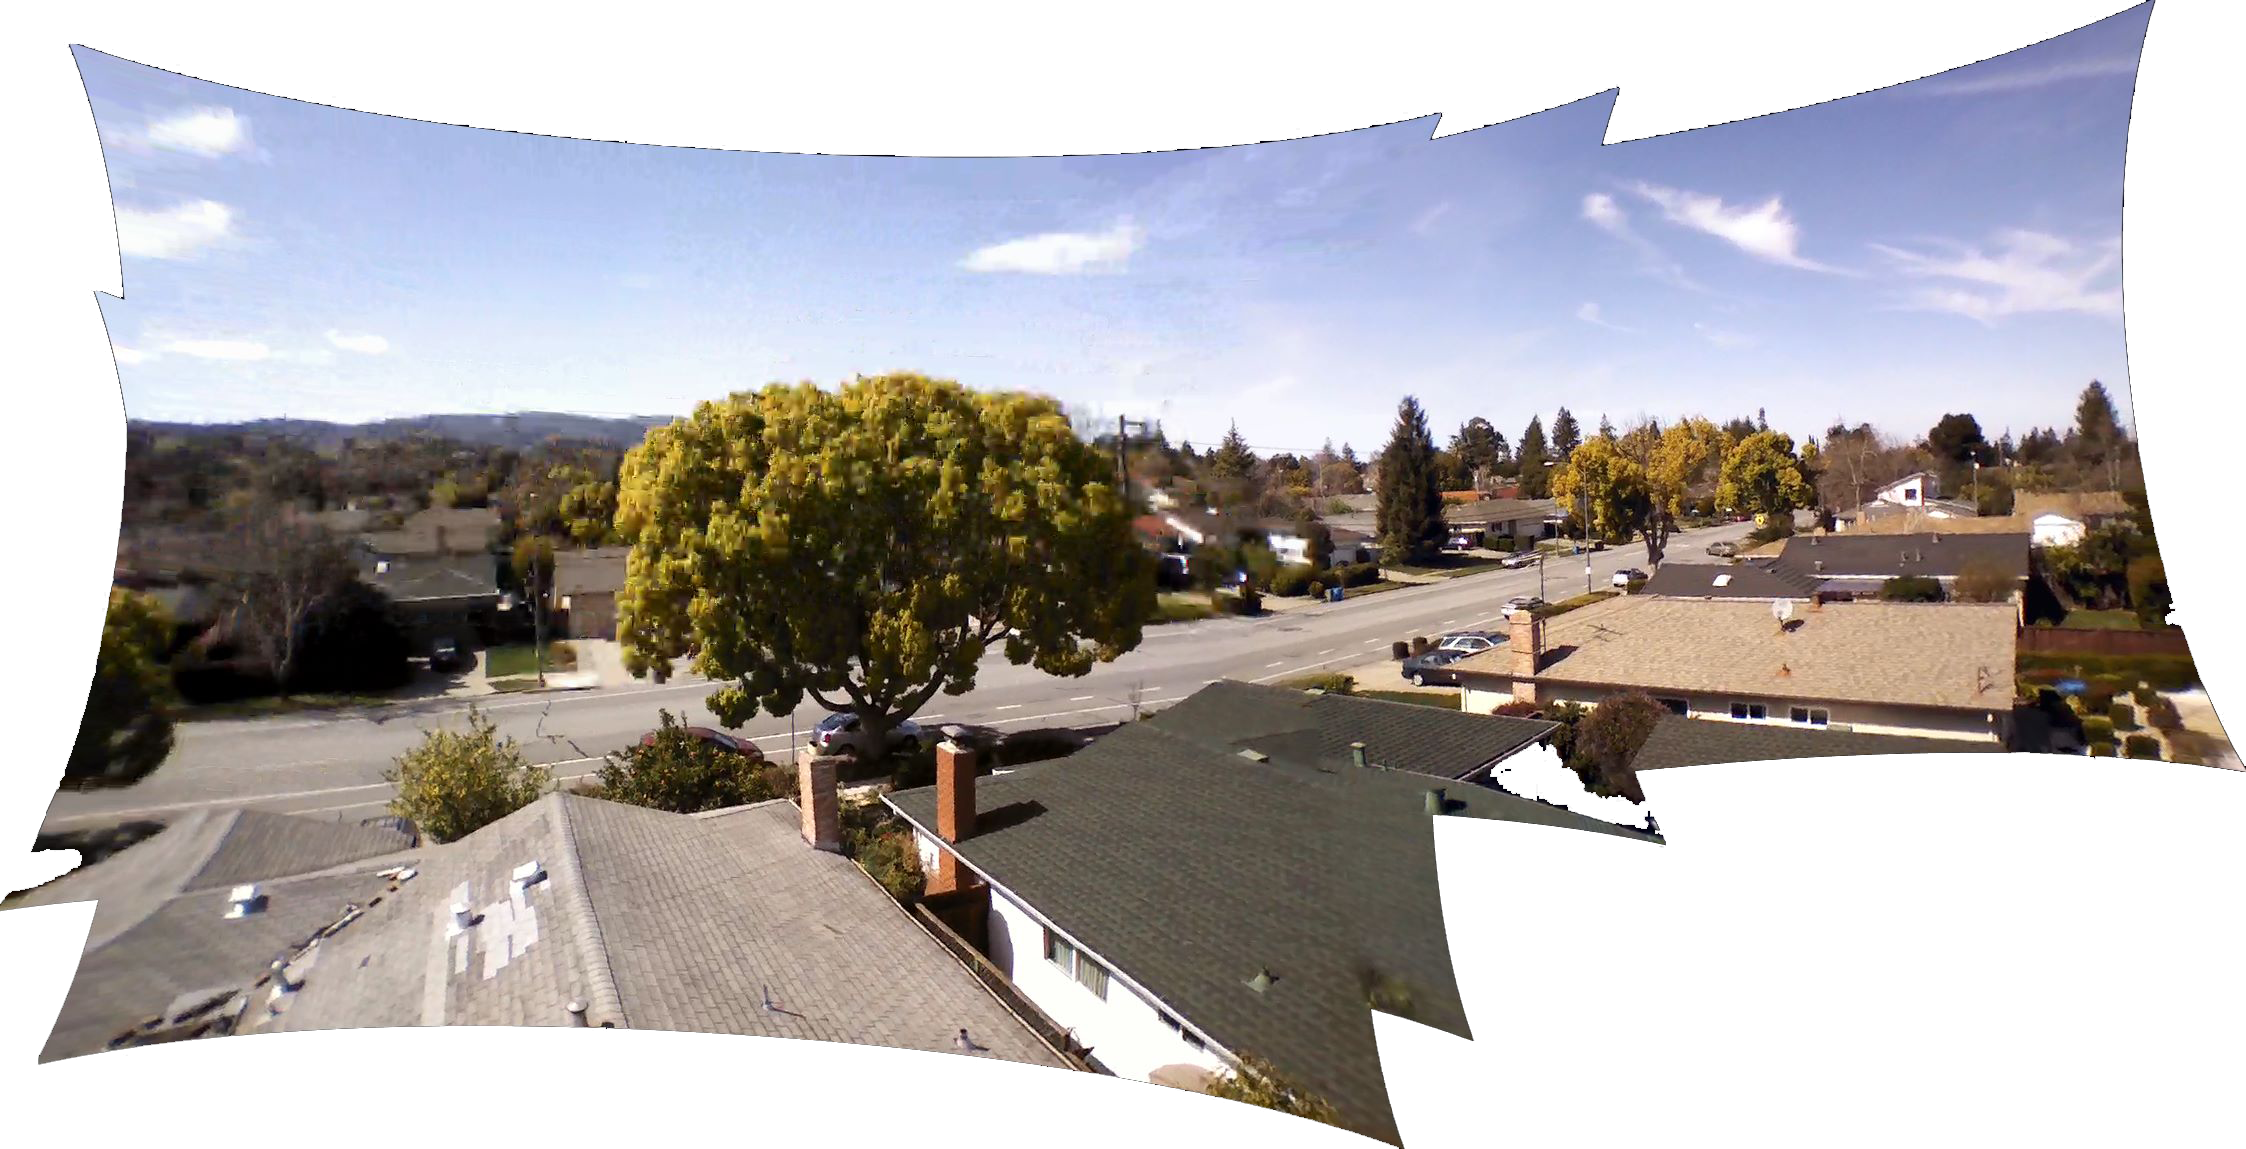
\includegraphics[width=\textwidth]{illustrations/maps/stelling}
\end{figure}


%\begin{figure}[H]
%	\caption{Stitch from low resolution stabilization camera}
%	\label{fig:BackyardStitch}
%	\centering
%		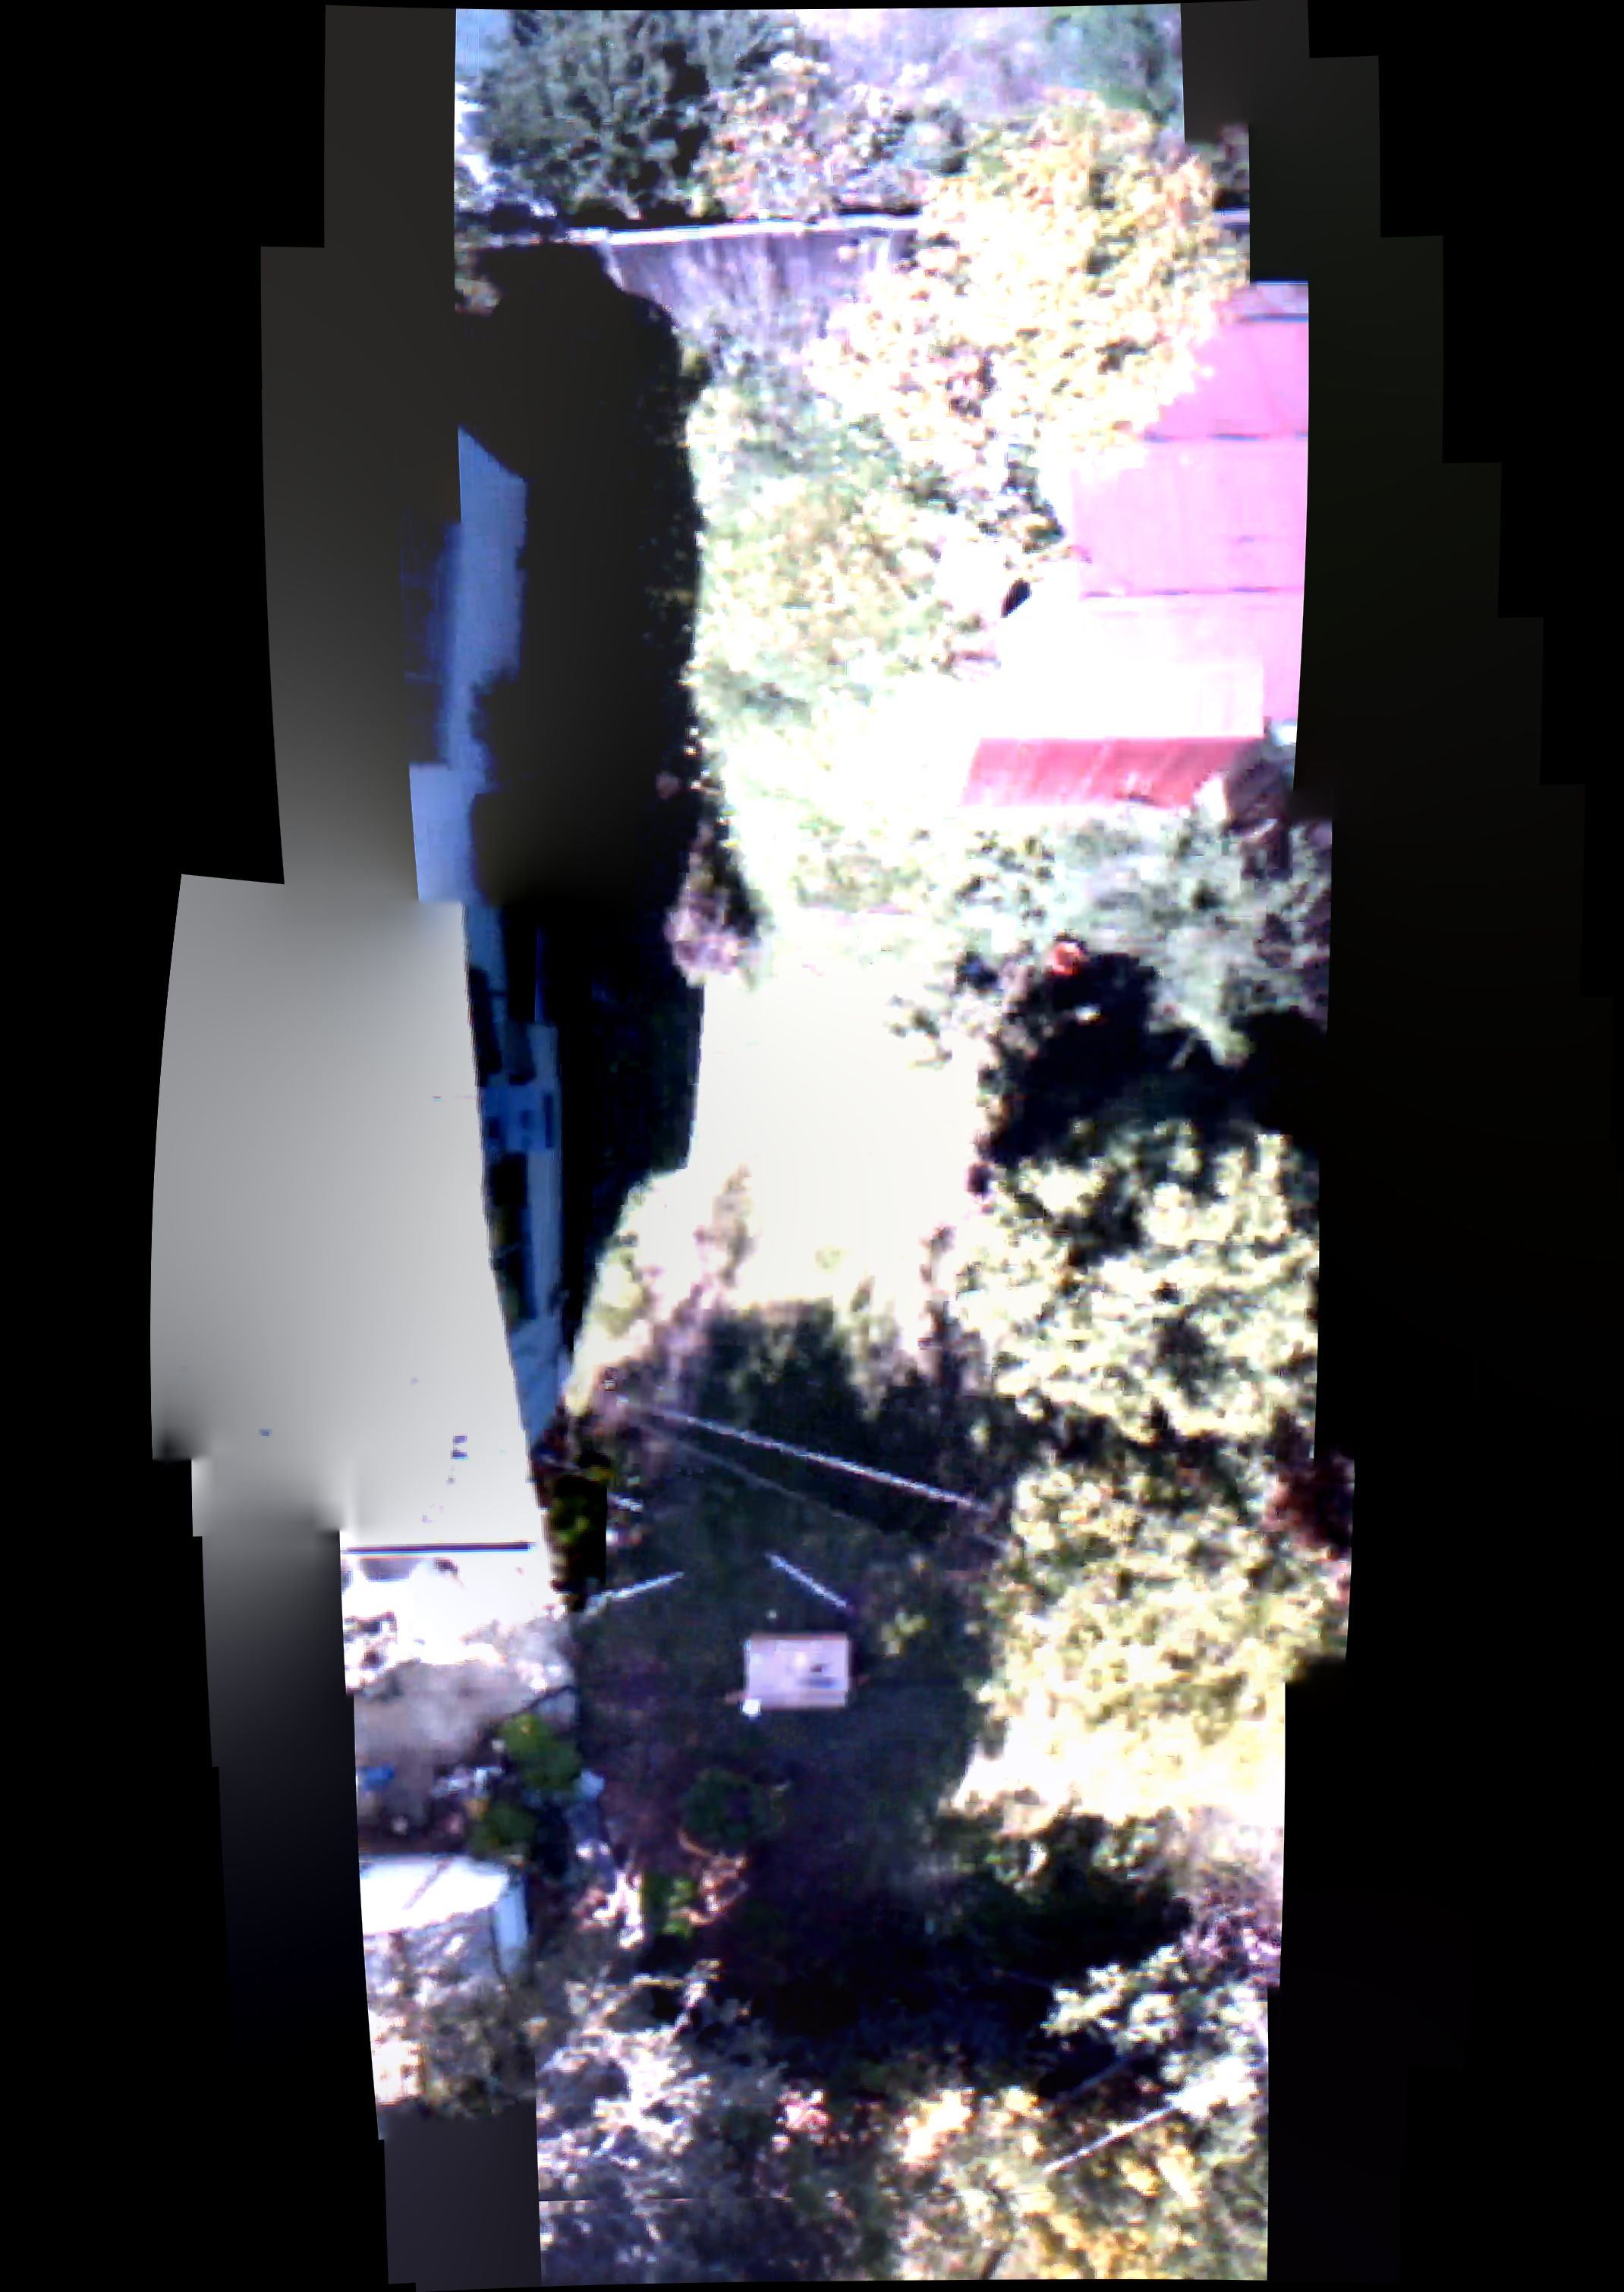
\includegraphics[width=.3\textwidth]{illustrations/maps/backyardOverhead2}
%\end{figure}